\documentclass{beamer}
\usetheme{default}
\usecolortheme{dove}
\usepackage{amsmath,amssymb}
\usepackage{tikz}
\usetikzlibrary{arrows.meta,positioning,calc}

\setbeamertemplate{navigation symbols}{}
\setbeamertemplate{footline}[frame number]

\title{Centered vs.\ Non-Centered MAP:\\Same Model, Different Optimization}
\author{}
\date{}

\begin{document}

\begin{frame}
\titlepage
\end{frame}

%% ============================================================
%% SLIDE: How ML Training Works
%% ============================================================
\begin{frame}{How ML Training Works (4 Steps, Every Epoch)}

\begin{center}
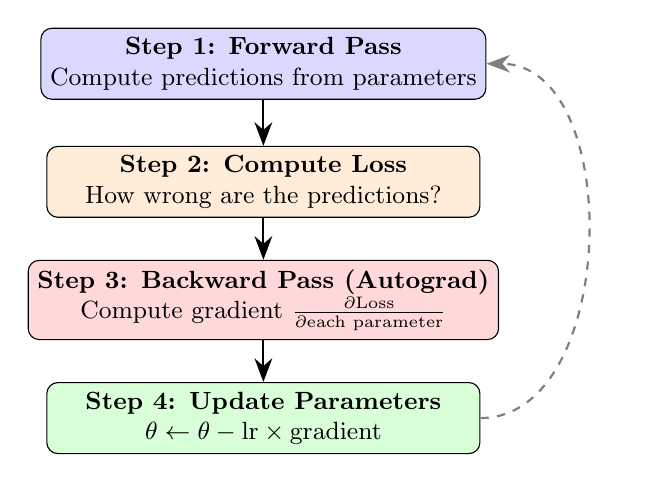
\begin{tikzpicture}[
    box/.style={rectangle, draw, rounded corners, minimum width=5.5cm, minimum height=0.9cm, font=\small, align=center},
    arr/.style={-{Stealth[length=3mm]}, thick}
]
    \node[box, fill=blue!15] (fwd) at (0,3) {\textbf{Step 1: Forward Pass}\\Compute predictions from parameters};
    \node[box, fill=orange!15] (loss) at (0,1.5) {\textbf{Step 2: Compute Loss}\\How wrong are the predictions?};
    \node[box, fill=red!15] (back) at (0,0) {\textbf{Step 3: Backward Pass (Autograd)}\\Compute gradient $\frac{\partial \text{Loss}}{\partial \text{each parameter}}$};
    \node[box, fill=green!15] (update) at (0,-1.5) {\textbf{Step 4: Update Parameters}\\$\theta \leftarrow \theta - \text{lr} \times \text{gradient}$};

    \draw[arr] (fwd) -- (loss);
    \draw[arr] (loss) -- (back);
    \draw[arr] (back) -- (update);
    \draw[arr, dashed, gray] (update.east) to[out=0,in=0] (fwd.east);
\end{tikzpicture}
\end{center}

\vspace{0.3cm}

\textbf{Key rule:} In Step 3, a parameter only gets a gradient from the loss if it was \textbf{used in Step 1} to compute the prediction. If a parameter isn't in the forward pass, autograd can't trace back to it.

\end{frame}

%% ============================================================
%% SLIDE: The Generative Model
%% ============================================================
\begin{frame}{The Generative Model (Same for Both)}

\begin{center}
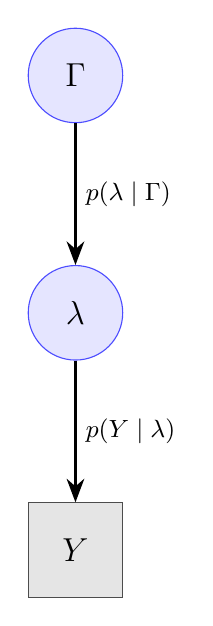
\begin{tikzpicture}[
    node distance=1.8cm,
    param/.style={circle, draw=blue!70, fill=blue!10, minimum size=1.2cm, font=\large},
    data/.style={rectangle, draw=black!70, fill=gray!20, minimum size=1.2cm, font=\large},
    arr/.style={-{Stealth[length=3mm]}, thick}
]
    \node[param] (gamma) {$\Gamma$};
    \node[param, below=of gamma] (lambda) {$\lambda$};
    \node[data, below=of lambda] (Y) {$Y$};

    \draw[arr] (gamma) -- node[right, font=\small] {$p(\lambda \mid \Gamma)$} (lambda);
    \draw[arr] (lambda) -- node[right, font=\small] {$p(Y \mid \lambda)$} (Y);
\end{tikzpicture}
\end{center}

\vspace{0.2cm}

\textbf{The joint distribution} (Giovanni's formulation):
\[
\lambda - G\Gamma \;\sim\; \mathcal{N}(0,\, K_\theta) \quad \Longleftrightarrow \quad p(\lambda \mid \Gamma) = \mathcal{N}(G\Gamma,\; K_\theta)
\]

\vspace{0.2cm}

\textbf{MAP loss} (identical in both parameterizations):
\[
\mathcal{L} = \underbrace{-\log p(Y \mid \lambda)}_{\text{NLL}} \;+\; \underbrace{W \|\delta\|^2_{K_\theta^{-1}}}_{\text{GP penalty on } \delta}
\]

where $\delta = \lambda - G\Gamma$. The GP penalizes $\delta$, not $\Gamma$ directly. $p(\Gamma) \propto 1$ (flat).

\end{frame}

%% ============================================================
%% SLIDE: The Prior on Gamma is Flat
%% ============================================================
\begin{frame}{The Prior on $\Gamma$ is Flat}

Factorize the hierarchy:
\[
p(Y,\lambda,\phi,\Gamma,\psi) = \underbrace{p(Y \mid \lambda,\phi,\psi)}_{\text{likelihood}} \cdot \underbrace{p(\lambda \mid \Gamma)}_{\text{GP on } \delta = \lambda - G\Gamma} \cdot \underbrace{p(\Gamma)}_{\propto\, 1}
\]

\vspace{0.3cm}

\begin{itemize}
    \item $p(\Gamma) \propto 1$ --- flat. No prior on $\Gamma$.
    \item $p(\lambda \mid \Gamma) = \mathcal{N}(\lambda;\; G\Gamma,\; K_\theta)$ --- this is the GP, and it's on $\delta$, not on $\Gamma$.
    \item The GP penalty in the MAP loss is $W \cdot \delta^\top K_\theta^{-1} \delta$. It penalizes $\delta$, not $\Gamma$.
\end{itemize}

\vspace{0.3cm}

\textbf{Key point:} The shrinkage of $\Gamma$ we observe in practice is \textbf{not} from a prior on $\Gamma$. It comes from optimization dynamics: during gradient descent, $\Gamma$ and $\delta$ compete to explain $\lambda$, and the GP penalty on $\delta$ shapes the landscape that $\Gamma$ optimizes over.

\vspace{0.3cm}

The \textbf{centered parameterization starves $\Gamma$ more} because the GP penalty has a direct gradient on $\Gamma$.

\end{frame}

%% ============================================================
%% SLIDE: The Centered Forward Pass
%% ============================================================
\begin{frame}{Centered Model: The Forward Pass}

\textbf{What the computer does each epoch:}

\vspace{0.4cm}

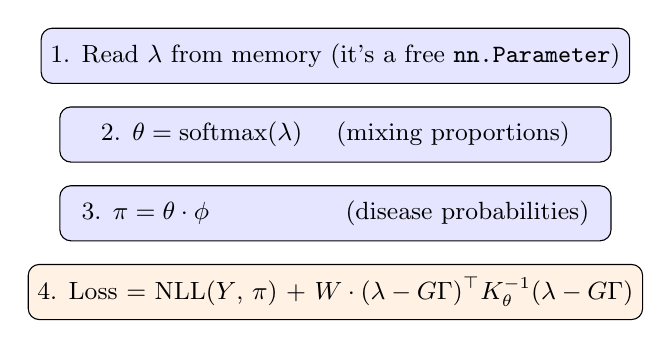
\begin{tikzpicture}[
    box/.style={rectangle, draw, rounded corners, minimum width=7cm, minimum height=0.7cm, font=\small, align=left},
]
    \node[box, fill=blue!10] (s1) at (0,3) {1. Read $\lambda$ from memory (it's a free \texttt{nn.Parameter})};
    \node[box, fill=blue!10] (s2) at (0,2) {2. $\theta = \text{softmax}(\lambda)$ \quad (mixing proportions)};
    \node[box, fill=blue!10] (s3) at (0,1) {3. $\pi = \theta \cdot \phi$ \quad\quad\quad\quad\quad (disease probabilities)};
    \node[box, fill=orange!10] (s4) at (0,0) {4. Loss = NLL($Y$, $\pi$) + $W \cdot (\lambda - G\Gamma)^\top K_\theta^{-1} (\lambda - G\Gamma)$};
\end{tikzpicture}

\vspace{0.5cm}

\textbf{Notice:} $\Gamma$ appears \textbf{only in the prior term} (Step 4), never in the forward computation (Steps 1--3).

\vspace{0.3cm}

$\lambda$ is read from memory $\rightarrow$ $\theta$ $\rightarrow$ $\pi$ $\rightarrow$ NLL. \\
The chain $Y \rightarrow \pi \rightarrow \theta \rightarrow \lambda$ does not pass through $\Gamma$.

\end{frame}

%% ============================================================
%% SLIDE: The Reparam Forward Pass
%% ============================================================
\begin{frame}{Non-Centered Model: The Forward Pass}

\textbf{What the computer does each epoch:}

\vspace{0.4cm}

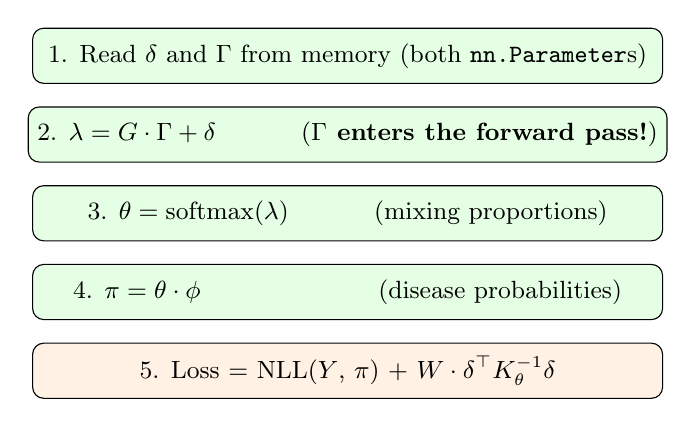
\begin{tikzpicture}[
    box/.style={rectangle, draw, rounded corners, minimum width=8cm, minimum height=0.7cm, font=\small, align=left},
]
    \node[box, fill=green!10] (s1) at (0,3) {1. Read $\delta$ and $\Gamma$ from memory (both \texttt{nn.Parameter}s)};
    \node[box, fill=green!10] (s2) at (0,2) {2. $\lambda = G \cdot \Gamma + \delta$ \quad\quad\quad (\textbf{$\Gamma$ enters the forward pass!})};
    \node[box, fill=green!10] (s3) at (0,1) {3. $\theta = \text{softmax}(\lambda)$ \quad\quad\quad (mixing proportions)};
    \node[box, fill=green!10] (s4) at (0,0) {4. $\pi = \theta \cdot \phi$ \quad\quad\quad\quad\quad\quad\; (disease probabilities)};
    \node[box, fill=orange!10] (s5) at (0,-1) {5. Loss = NLL($Y$, $\pi$) + $W \cdot \delta^\top K_\theta^{-1} \delta$};
\end{tikzpicture}

\vspace{0.5cm}

\textbf{Now:} $\Gamma$ is \textbf{in the forward computation} (Step 2). \\
The chain is: $\Gamma \rightarrow \lambda \rightarrow \theta \rightarrow \pi \rightarrow$ NLL.

\vspace{0.3cm}

Autograd traces back through this chain, so $\Gamma$ gets a gradient from the data.

\end{frame}

%% ============================================================
%% SLIDE: The Backward Pass — Gradient Comparison
%% ============================================================
\begin{frame}{The Backward Pass: Gradient Comparison}

\textbf{Centered model:}
\[
\frac{\partial \mathcal{L}}{\partial \Gamma_k} = \underbrace{\overset{{\color{red}\mathbf{= 0}}}{\frac{\partial \text{NLL}}{\partial \Gamma_k}}}_{\text{\color{red} Not in forward pass!}} + \underbrace{W \cdot (-2) \sum_i G_i^\top K_\theta^{-1} \delta_{ik}}_{\text{\color{blue} prior only ($W$=1e-4, weak)}}
\]

\pause
\vspace{0.2cm}
\hrule
\vspace{0.2cm}

\textbf{Non-centered model:}
\[
\frac{\partial \mathcal{L}}{\partial \Gamma_k} = \underbrace{\frac{\partial \text{NLL}}{\partial \pi} \cdot \frac{\partial \pi}{\partial \theta} \cdot \frac{\partial \theta}{\partial \lambda} \cdot G^\top}_{\text{\color{green!60!black} chain rule through forward pass (strong!)}} + \; \underbrace{0}_{\text{$\delta$ indep.\ of $\Gamma$}}
\]

\vspace{0.3cm}

\textbf{Same loss, different gradient pathways:}
\begin{itemize}
    \item Centered: $\Gamma$ gets a direct GP penalty gradient that \textbf{shrinks} it ($\propto W \cdot G^\top K^{-1}\delta$), but \textbf{no} NLL gradient --- the data can't speak to $\Gamma$
    \item Non-centered: $\Gamma$ gets \textbf{zero} GP penalty gradient, but a \textbf{strong} NLL gradient --- the data drives $\Gamma$ directly
\end{itemize}

\end{frame}

%% ============================================================
%% SLIDE: Same Objective, Different Computation
%% ============================================================
\begin{frame}{Same Objective, Different Computation}

Both models minimize the \textbf{same function}:
\[
\mathcal{L} = -\log p(Y \mid \lambda) + W\|\lambda - G\Gamma\|^2_{K_\theta^{-1}}
\]

\pause
\vspace{0.2cm}

The difference is purely in \textbf{how the computer represents $\lambda$}:

\vspace{0.3cm}

\begin{tabular}{l|c|c}
 & \textbf{Centered} & \textbf{Non-centered} \\ \hline
\rule{0pt}{2.5ex}Free parameters & $\lambda$, $\Gamma$ & $\delta$, $\Gamma$ \\[4pt]
Forward pass & $\theta = \text{softmax}(\lambda)$ & $\lambda = G\Gamma + \delta$ \\
 & & $\theta = \text{softmax}(\lambda)$ \\[4pt]
GP gradient on $\Gamma$ & Nonzero (but $\propto W$) & Zero \\[4pt]
NLL gradient on $\Gamma$ & \color{red}{Zero} & \color{green!60!black}{Strong (chain rule)} \\[2pt]
Net effect on $\Gamma$ & Over-shrunk & Well-estimated \\
\end{tabular}

\vspace{0.4cm}

\textbf{At any solution:} $\delta^* = \lambda^* - G\Gamma^*$. If the problem were convex, both would find the same optimum. It is \textbf{non-convex}: different gradient flows $\rightarrow$ different local optima.

\end{frame}

%% ============================================================
%% SLIDE: The Gradient Flow Picture
%% ============================================================
\begin{frame}{The Gradient Flow Picture}

\begin{columns}
\column{0.48\textwidth}
\textbf{Centered:}
\begin{center}
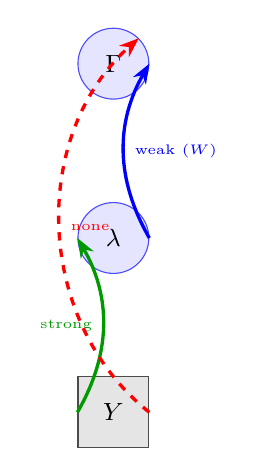
\begin{tikzpicture}[
    node distance=1.3cm,
    param/.style={circle, draw=blue!70, fill=blue!10, minimum size=0.9cm, font=\small},
    data/.style={rectangle, draw=black!70, fill=gray!20, minimum size=0.9cm, font=\small},
    grad/.style={-{Stealth[length=2.5mm]}, very thick},
]
    \node[param] (gamma) {$\Gamma$};
    \node[param, below=of gamma] (lambda) {$\lambda$};
    \node[data, below=of lambda] (Y) {$Y$};

    \draw[grad, green!60!black] (Y.west) to[bend right=30] node[left, font=\tiny, text=green!60!black] {strong} (lambda.west);
    \draw[grad, blue] (lambda.east) to[bend left=30] node[right, font=\tiny, text=blue] {weak ($W$)} (gamma.east);
    \draw[grad, red, dashed] (Y.east) to[bend left=50] node[right, font=\tiny, text=red] {none} (gamma.north east);
\end{tikzpicture}
\end{center}

\column{0.48\textwidth}
\textbf{Non-centered:}
\begin{center}
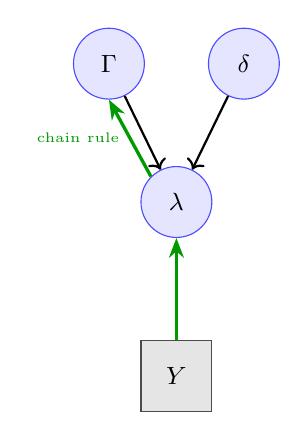
\begin{tikzpicture}[
    node distance=1.3cm,
    param/.style={circle, draw=blue!70, fill=blue!10, minimum size=0.9cm, font=\small},
    data/.style={rectangle, draw=black!70, fill=gray!20, minimum size=0.9cm, font=\small},
    grad/.style={-{Stealth[length=2.5mm]}, very thick},
]
    \node[param] (gamma) {$\Gamma$};
    \node[param, right=0.8cm of gamma] (delta) {$\delta$};
    \node[param, below=1.3cm of $(gamma)!0.5!(delta)$] (lambda) {$\lambda$};
    \node[data, below=of lambda] (Y) {$Y$};

    \draw[thick, ->] (gamma) -- (lambda);
    \draw[thick, ->] (delta) -- (lambda);
    \draw[grad, green!60!black] (Y) -- (lambda);
    \draw[grad, green!60!black] (lambda.north west) -- node[left, font=\tiny, text=green!60!black] {chain rule} (gamma.south);
\end{tikzpicture}
\end{center}
\end{columns}

\vspace{0.5cm}

Both $\Gamma$ and $\delta$ feed into $\lambda$ in the forward pass $\rightarrow$ both get NLL gradients.

In centered, $\lambda$ is a dead-end: NLL gradients stop there and never reach $\Gamma$.

\end{frame}

%% ============================================================
%% SLIDE: Simulation Evidence
%% ============================================================
\begin{frame}{Simulation: $\gamma$ Recovery}

\textbf{Parameter recovery simulation} (10k patients, 10 PRS, 5 signatures):

\vspace{0.3cm}

\begin{center}
\begin{tabular}{l|c|c|c}
 & \textbf{Centered} & \textbf{Reparam ($\kappa$ free)} & \textbf{Nokappa ($\kappa=1$)} \\ \hline
\rule{0pt}{2.5ex}$r(\hat\gamma, \gamma_{\text{true}})$ & 0.796 & 0.953 & 0.954 \\
Mean $|\hat\gamma|$ & 0.175 & 0.197 & 0.191 \\
True mean $|\gamma|$ & \multicolumn{3}{c}{0.200} \\
\end{tabular}
\end{center}

\vspace{0.3cm}

\begin{itemize}
    \item Non-centered recovers $\gamma$ with $r = 0.954$ vs.\ $r = 0.796$ for centered
    \item Both show mild shrinkage (estimated $|\gamma|$ slightly below true)
    \item Residual shrinkage in non-centered is an \textbf{optimization phenomenon}: $\Gamma$ and $\delta$ jointly determine $\lambda$, and the GP penalty on $\delta$ shapes the landscape $\Gamma$ optimizes over
    \item $\kappa$ free vs.\ fixed at 1: essentially no difference ($r = 0.953$ vs $0.954$)
\end{itemize}

\end{frame}

%% ============================================================
%% SLIDE: Stability Across Batches
%% ============================================================
\begin{frame}{$\gamma$ Stability Across 40 Training Batches}

\small

\begin{center}
\begin{tabular}{l|c|c}
 & \textbf{Non-centered} & \textbf{Centered} \\ \hline
\rule{0pt}{2.5ex}Mean $|\gamma|$ (pooled) & 0.065 & 0.005 \\
Mean batch std & 0.136 & 0.015 \\
Median CV & 2.50 & 5.91 \\
Sign-flip rate & 30\% & 39\% \\
Batch-to-mean correlation & 0.48 & 0.58 \\
\end{tabular}
\end{center}

\vspace{0.3cm}

\textbf{Key biological signals are stable} (boxplot across 40 batches):
\begin{itemize}
    \item T2D $\to$ Sig 15 (DM): consistently $\sim 1.2$, tight box, never crosses zero
    \item CAD $\to$ Sig 5 (Ischemic CVD): consistently $\sim 0.25$, all positive
    \item BMI $\to$ Sig 7 (Metabolic): all positive, tight range
\end{itemize}

\vspace{0.2cm}

The high median CV is driven by weak/noise entries. \textbf{Pooling across batches} regularizes $\gamma$ by $\sqrt{B}$, acting as the post-hoc equivalent of the implicit prior.

\end{frame}

%% ============================================================
%% SLIDE: Psi Stability
%% ============================================================
\begin{frame}{$\psi$ Stability: Much More Consistent}

\begin{center}
\begin{tabular}{l|c|c}
 & \textbf{$\gamma$ (genetics $\to$ sigs)} & \textbf{$\psi$ (sigs $\to$ diseases)} \\ \hline
\rule{0pt}{2.5ex}Median CV & 2.50 & 0.14 \\
Sign-flip rate & 30\% & 2.4\% \\
Batch-to-mean corr & 0.48 & 0.96 \\
\end{tabular}
\end{center}

\vspace{0.3cm}

\textbf{Why is $\psi$ more stable?}
\begin{itemize}
    \item $\psi$'s tradeoff partner is $\epsilon$ (shared across all $N$ patients)
    \item $\gamma$'s tradeoff partner is $\delta$ (per-patient, $N \times K \times T$ free parameters)
    \item $\delta$ has more flexibility to absorb signal that $\gamma$ would explain
    \item $\epsilon$ is constrained to work for all patients simultaneously
\end{itemize}

\vspace{0.3cm}

\textbf{Psi switches from initialization:} only 9/348 diseases changed max signature --- all biologically reasonable reassignments.

\end{frame}

%% ============================================================
%% SLIDE: Prediction AUC
%% ============================================================
\begin{frame}{Prediction AUC: Centered vs.\ Non-Centered}

\small
LOO evaluation: pool parameters from training batches, fit $\delta$ on held-out patients:

\vspace{0.3cm}

\begin{center}
\begin{tabular}{l|c|c|c}
\textbf{Metric} & \textbf{Centered (nolr)} & \textbf{Non-centered} & \textbf{$\Delta$} \\ \hline
\rule{0pt}{2.5ex}Static 10-year & 0.622 & 0.654 & +0.032 \\
Dynamic 10-year & 0.624 & 0.629 & +0.005 \\
Dynamic 1-year & 0.765 & 0.883 & +0.118 \\
Static 1-year & 0.770 & 0.878 & +0.108 \\
\end{tabular}
\end{center}

\vspace{0.3cm}

\textbf{Non-centered wins on all metrics}, especially short-horizon:
\begin{itemize}
    \item The genetically-informed prior mean $G\Gamma$ gives different starting points for high-risk vs.\ low-risk patients (\textbf{between-strata} discrimination)
    \item $\delta$ captures individual residual variation (\textbf{within-strata} discrimination)
    \item Centered model had to do both with a single $\lambda$
\end{itemize}

\end{frame}

%% ============================================================
%% SLIDE: Why Centered Starves Gamma
%% ============================================================
\begin{frame}{Why the Centered Model Starves $\Gamma$}

\textbf{Centered:} $\lambda$ is the free parameter, $\delta = \lambda - G\Gamma$ is derived.

The GP penalty gradient w.r.t.\ $\Gamma_k$:
\[
\nabla_{\Gamma_k} \text{GP} = -2W \sum_{i} G_i^\top K_\theta^{-1} \underbrace{(\lambda_{ik} - G_i\Gamma_k)}_{\delta_{ik}}
\]

This is \textbf{nonzero} --- it directly regularizes $\Gamma$ toward values where $\delta \to 0$.

\vspace{0.3cm}
\hrule
\vspace{0.3cm}

\textbf{Non-centered:} $\delta$ is the free parameter, $\lambda = G\Gamma + \delta$.

The GP penalty is $W \cdot \delta^\top K^{-1} \delta$. Its gradient w.r.t.\ $\Gamma_k$:
\[
\nabla_{\Gamma_k} \text{GP} = 0
\]

\textbf{Zero.} $\delta$ doesn't depend on $\Gamma$. No penalty touches $\Gamma$.

\vspace{0.3cm}

$\Gamma$ only sees the NLL gradient via the chain rule $Y \to \pi \to \theta \to \lambda \to \Gamma$. The data speaks directly to $\Gamma$ without competition from a prior penalty.

\end{frame}

%% ============================================================
%% SLIDE: A Simple Analogy
%% ============================================================
\begin{frame}{A Simple Analogy}

Minimize $f(x) = (x - 3)^2$ with a preference that $x$ be near $\mu$:

\vspace{0.3cm}

\textbf{Centered:}
\begin{itemize}
    \item Parameters: $x$ and $\mu$
    \item Loss $= (x-3)^2 + w \cdot (x - \mu)^2$
    \item $\mu$ only appears in the penalty. If $w$ is small, $\mu$ barely moves.
\end{itemize}

\vspace{0.3cm}

\textbf{Non-centered:}
\begin{itemize}
    \item Parameters: $z$ and $\mu$, where $x = \mu + z$
    \item Loss $= (\mu + z - 3)^2 + w \cdot z^2$
    \item $\mu$ appears in the \textbf{main loss}. It gets a strong gradient.
\end{itemize}

\vspace{0.3cm}

Same model, same answer ($x^* = 3$), but in the non-centered form $\mu$ learns where $x$ wants to be. In the centered form, $\mu$ barely moves because $w$ is tiny.

\end{frame}

%% ============================================================
%% SLIDE: Summary
%% ============================================================
\begin{frame}{Summary}

\begin{enumerate}
    \item \textbf{Same model, flat prior on $\Gamma$:} $p(\Gamma) \propto 1$. The GP prior is on $\delta = \lambda - G\Gamma$, not on $\Gamma$.

    \vspace{0.2cm}

    \item \textbf{Centered starves $\Gamma$:} GP penalty has a direct gradient on $\Gamma$ that shrinks it; the NLL has no gradient on $\Gamma$ at all. Non-centered: GP gradient on $\Gamma$ is zero; NLL gradient is strong.

    \vspace{0.2cm}

    \item \textbf{Simulation:} Non-centered recovers $\gamma$ with $r = 0.954$ vs.\ $0.796$ for centered. Residual shrinkage in non-centered is an optimization phenomenon, not a prior.

    \vspace{0.2cm}

    \item \textbf{Real data:} Key biological signals (T2D, CAD, BMI) are stable across 40 batches. $\psi$ is very stable (CV = 0.14). Pooling regularizes $\gamma$.

    \vspace{0.2cm}

    \item \textbf{Prediction:} Non-centered wins on all AUC metrics (+0.118 on dynamic 1-year). Genetically-informed $G\Gamma$ provides between-strata discrimination; $\delta$ handles within-strata.

    \vspace{0.2cm}

    \item \textbf{Standard approach:} Non-centered parameterization is the classical alternative in hierarchical models (Stan, PyMC) when data is informative about group-level parameters.
\end{enumerate}

\end{frame}

\end{document}
